% -----------------------------------------------
% Template for ISMIR 2014
% (based on earlier ISMIR templates)
% -----------------------------------------------

\documentclass{article}
\usepackage{ismir2014,amsmath,cite}
\usepackage{graphicx}
\usepackage{multirow}
\usepackage{units}

% Title.
% ------
\title{DRUM TRANSCRIPTION IN POLYPHONIC MUSIC USING SEMI-SUPERVISED NON-NEGATIVE MATRIX FACTORIZATION}

% Single address
% To use with only one author or several with the same address
% ---------------
%\oneauthor
% {Names should be omitted for double-blind reviewing}
% {Affiliations should be omitted for double-blind reviewing}

% Two addresses
% --------------
%\twoauthors
%  {First author} {School \\ Department}
%  {Second author} {Company \\ Address}

% Three addresses
% --------------
\threeauthors
  {First author} {Affiliation1 \\ {\tt author1@ismir.edu}}
  {Second author} {\bf Retain these fake authors in\\\bf submission to preserve the formatting}
  {Third author} {Affiliation3 \\ {\tt author3@ismir.edu}}

% Four addresses
% --------------
%\fourauthors
%  {First author} {Affiliation1 \\ {\tt author1@ismir.edu}}
%  {Second author}{Affiliation2 \\ {\tt author2@ismir.edu}}
%  {Third author} {Affiliation3 \\ {\tt author3@ismir.edu}}
%  {Fourth author} {Affiliation4 \\ {\tt author4@ismir.edu}}

\begin{document}
%
\maketitle
%
\begin{abstract}
In this paper, a drum transcription algorithm using semi-supervised non-negative matrix factorization has been presented. This method allows users to separate percussive activities from harmonic activities with pre-trained drum templates, and detect drum events from the extracted percussive activity matrix. A polyphonic subset from ENST drum dataset has been used for training and testing of the algorithm. The system has been tested using different rank settings, and a cross-performer validation process has been performed to evaluate the reliability of the system.  The results show that the system can achieve 61 to 77\% recognition rate on multiple drums in polyphonic music. In the future, more efforts will be put on differentiating different playing styles and more drum parts, leading toward a complete drum transcription system.

\end{abstract}
%

\section{Introduction}\label{sec:introduction}
Transcribing music content into sheet music or any form of score is an essential skill to musicians for analysis and composition purposes. However, It is often considered a time-consuming and non-trivial task, for it requires repetitive listening and integral knowledge of music and instruments. With the advance of computing power and various machine learning techniques, a system that has the abilities to automatically recognize music content has become a plausible idea and interests many researchers in the field of Music Information Retrieval (MIR) \cite{1}. In general, Automatic Music Transcription (AMT) systems could not only serve as a tool to record the music content, identify notes from improvisations, but also lead to the realization of a music intelligence system \cite{2}. To build a complete AMT system, many subtasks and challenges, such as multi-pitch detection, onset detection, instrument recognition, and rhythm extraction, have been attempted [1]. Comparing with pitched instruments, transcribing un-pitched music events such as percussive sounds seem to be less addressed, and a robust algorithm to detect drum sounds in polyphonic music is still an open question in this field.

Drum track, especially in pop music, often plays an important role in determining music structure, style, rhythm and tempo. In many cases, it shares the same importance as the harmonic part in the music. That said, a good drum transcription system could provide essential information of the music content, and could potentially facilitate the realization of many interesting applications. For example, a drum transcription and drum source separation task could mutually benefit from each other and provide the possibility to manipulate drum sounds within an existing drum track \cite{3,4}.  Also, music education could be an application of a drum transcription system, for it could help students identify drum event within a polyphonic music, and provide instructions by analyzing and comparing the differences between the input and reference performances. Furthermore, such system could also be integrated as a part of machine listening, improving the existing systems of robotic musicians \cite{5}.

Therefore, this study aims to explore alternative solutions to drum transcription in polyphonic music. The final goal of this paper is to find a potential direction to push the limit of this task, leading toward further musical applications.

\section{Related Work}\label{sec:related works}
The early attempts to transcribe percussive sounds main focused on classifying monophonic signals \cite{6,7}. With standard approaches such as feature extraction and classification, fairly high accuracy were reported in the previous studies. However, in the real use case, a drum transcription system is expected to work in polyphonic signal instead of monophonic. Therefore, solving this problem in the context of polyphonic music had become another criterion, and different methods could be found in previous research \cite{8,9,10,11,12,13,14,15}.  According to \cite{15}, recent studies on the drum transcription in polyphonic music could be categorized into three types: segment and classify, separate and detect, match and adapt.  For the first type of approaches, the common procedure starts by applying onset detection to the audio signal in order to segment the music event. Once the event has been detected, various features from time or spectral domain of the signal will be extracted, and a classifier will be trained to classify the event based on the extracted features. This type of approaches seem to perform well when the data and features are well chosen \cite{13,15}. However, to get good results, sufficient amount of data, careful preprocessing and training steps are required in this type of systems. Additionally, to handle the situation of simultaneous sounds, more classes need to be trained.

The second type of approaches is based on the assumption that music signal is a superposition of different sound sources. By decomposing the signal and into different source templates and corresponding activities, the music content could be transcribed by detecting onsets of these activities. Different methods such as Independent Subspace Analysis (ISA) \cite{16}, Prior Subspace Analysis (PSA) \cite{8}, and Non-negative Matrix Factorization (NMF) \cite{14,17,18} are the examples in this category. This type of approaches is usually easier to interpret, since most of the decompositions have been done on the spectrogram of the signal. Also, the separate nature allows simultaneous events to be handled easily in this case. However, to be able to transcribe different kinds of music, a large template might be required prior to the decomposition. Moreover, the number of rank during the decomposition process could be difficult to determine in some cases. 

The third type of approaches uses pre-trained templates to detect drum events \cite{19,20}. An iterative process has been taken to search for the closest matches to these templates and adapt them. The proposed system has been evaluated and performed well in MIREX 2005 drum detection competition. However, to coverage a wider range of sounds, multiple seed templates need to be prepared prior to the process.

In this paper, a method based on the NMF approach has been presented. Although NMF has been proven to be effective in music transcription (\cite{2003 Smaragdis, NMF}), it is still difficult to determine the number of sources in the target signal for a correct rank parameter setting. Therefore, the goal of this paper is to develop an algorithm that provides a more general use case, which only requires users to input a few drum samples prior to the decomposition process. This method aims to serve as an alternative way to transcribe drum tracks in polyphonic music, leading toward an end user application for general drum transcription tasks.  
 
\section{Method}\label{sec:method}
\subsection{Algorithm Description}\label{subsec:algorithm description}
% introduce NMF here
The basic concept of NMF is to approximate a non-negative matrix $V$ with two non-negative matrix $W$ and $H$ as shown in equation \eqref{eq:approx}.

% equation here
\begin{equation}
V \approx WH
\label{eq:approx}
\end{equation}

That is, given a $m \times n$ matrix $V$, the NMF will decompose the matrix into the product of a $m \times r$ matrix $W$ and a $r \times n$ matrix $H$. The $r$ is the rank of the NMF decomposition, $W$ is the basis matrix, and $H$ is the activity matrix. In the case of spectrogram, $V$ is the spectrogram to be decomposed, $W$ would be the spectra of the salient components, and $H$ would be the activity of these components respect to time. These matrices could be obtained through an iterative process to minimize the distance measure between the approximate and target spectrograms using the algorithm described in (\cite{} algorithm NMF 2001). 

To apply this method directly to the transcription tasks, however, some situations need to be taken into consideration. First of all, in the real situation, the number of sound sources within a recording is unknown. That said, it is very difficult to set a correct rank number and obtain a clear representation of the decomposed  components. Secondly, when the rank number is high, it is hard to identify the corresponding instrument of every component in the basis matrix $W$. To address these issues, different methods have been proposed in the previous studies. In (\cite{} Virtanen 2005), a SVM was trained to separate drum components from the harmonic components with a empirically set rank number during the factorization process. The identified drum components and their corresponding activities could later be used to reconstruct the drum signal, achieving the goal of drum source separation. However, this method requires separated data to train the classifier, and the results could be data-dependent. In (\cite{} co-factorization 2010), a co-factorization algorithm was proposed to simultaneously factorize a target signal a the drum track, and use the basis matrix from the drum track to identify the drum components in the target signal. This method ensures the drum components in both basis matrices to be the same over the iterations, thus, the harmonic parts could be isolated by removing the drum components. The need to obtain a drum track prior to the factorization process, however, could be difficult in many application scenarios.

%============= Factorization figure
\begin{figure}
 \centerline{\framebox{
 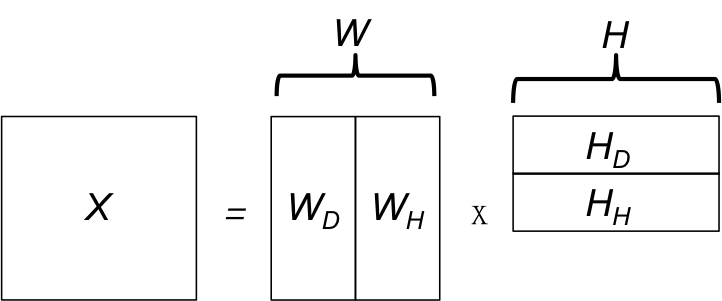
\includegraphics[width=\columnwidth]{factorization.png}}}
 \caption{Illustration on the factorization process. The $W_D$ is a pre-trained drum basis matrix, and it will not be updated over the iterations }
 \label{fig:factorization}
\end{figure}

% introduce my modification here 
In this paper, a method based on (\cite{} co-factorization 2010) has been proposed to remove the requirement the prior drum track. As shown in \figref{fig:factorization}, assuming a signal contains drum and harmonic parts, its spectrogram could be decomposed into basis matrix $W$ and activity matrix $H$. In this case, the $W$ consists of $W_D$ and $W_H$, and the $H$ consists of $H_D$ and $H_H$, respectively. Here, we first initialize $W_D$ with drum templates to be detected. Next, given an arbitrary rank number, the $W_H$, $H_H$, and $H_D$ could be initialized with random numbers. An iterative process is taken to minimize the cost function as shown in equation \eqref{eq:costFunc}. By applying gradient decent and multiplicative update rules, the matrices could be updated by the equation \eqref{eq:updateHD} \eqref{eq:updateWH} \eqref{eq:updateHH}, and the corresponding drum events could be detected from $H_D$.  
% equation here
\begin{equation}
C = \frac{1}{2} || X - W_{D}H_{D} - W_{H}H_{H}||^{2}
\label{eq:costFunc}
\end{equation}

% equation here
\begin{equation}
H_{D} \leftarrow H_{D}\frac{W_{D} ^T X}{W_{D}^T W_{D} H_{D} + W_{D} W_{H} H_{H}}
\label{eq:updateHD}
\end{equation}

% equation here
\begin{equation}
W_{H} \leftarrow W_{H}\frac{X H_{H}^T}{W_{H} H_{H} H_{H}^T + W_{D} H_{D} H_{H}^T}
\label{eq:updateWH}
\end{equation}

% equation here
\begin{equation}
H_{H} \leftarrow H_{H}\frac{W_{H}^T X}{W_{H}^T W_{H} H_{H} + W_{H} W_{D} H_{D}}
\label{eq:updateHH}
\end{equation}\\


Finally, the method described above can be summarized as the following steps:
\begin{enumerate}
    \item   Construct a $m \times r$ drum basis matrix $W_D$, $H_r$ is the number of drum components to be detected.
    \item   Given a fixed rank $k$, initialize a $m \times k$ matrix $W_H$, a $r \times n$ matrix $H_D$ and a $k \times n$ matrix $H_H$.
    \item   Normalize $W_D$ and $W_H$.
    \item   Update $H_D$, $W_H$, and $H_H$ using equation \eqref{eq:updateHD}, \eqref{eq:updateWH} and \eqref{eq:updateHH}.
    \item   Calculate the cost of current iteration using equation \eqref{eq:costFunc}.
    \item   Repeat step 2 to step 5 until it converges.
\end{enumerate}

\subsection{Processing Steps}\label{subsec:processing steps}

The system flowchart is shown in \figref{fig:flowchart}. The basic setup is shown on the right hand side. The STFT of the signals will be first calculated using a window size = 2048 and a hop size = 512. A pre-trained drum basis matrix will be constructed from the training data of single drum sounds. Next, the semi-supervised NMF will be performed with a given rank $k$. Finally, in the onset detection stage, the drum activity matrix will be used as novelty functions to determine the onset positions and their corresponding classes.  

The grey area in \figref{fig:flowchart} is another optional setup of the drum transcription system. To enhance the performance on hihat detection, the testing music signal and the training drum samples will be passed into a 2nd order Butterworth high-pass filter first. The cutoff frequency is derived from the average spectrum of the training drum samples and is set to \unit[8000]{Hz}. The extracted activity matrix from this part is used only for hihat detection. More details on the template extraction and activity detection will be elaborated in the following sections. 

%============= System + high pass figure here
\begin{figure}
 \centerline{\framebox{
 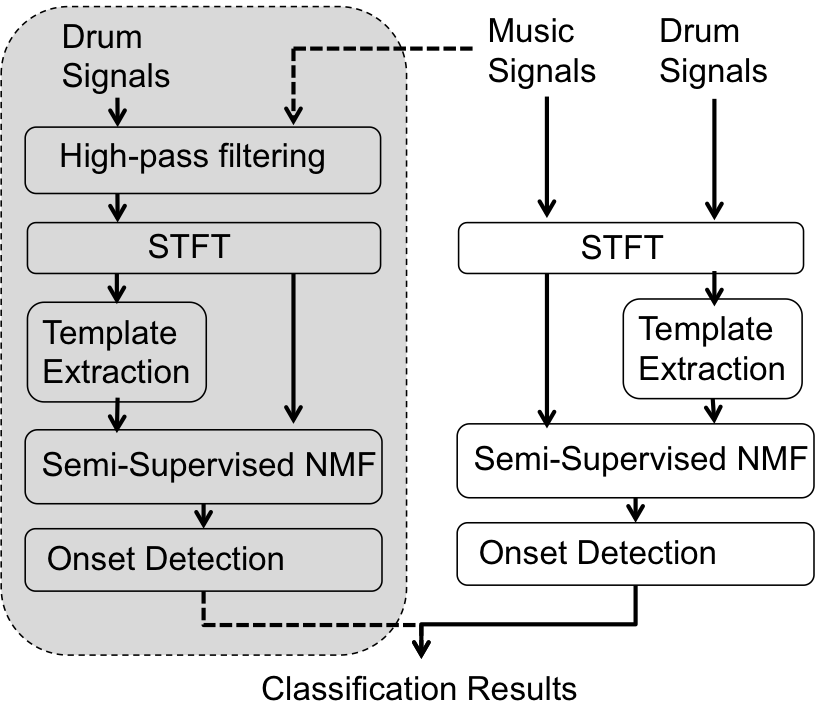
\includegraphics[width=\columnwidth]{flowchart.png}}}
 \caption{Flowchart of the drum transcription system.}
 \label{fig:flowchart}
\end{figure}

\subsubsection{Template Extraction}\label{subsubsec:template extraction}
The drum basis matrix is created by extracting template spectrum from the training drum samples. To extract the template spectrum for one class of drum, all the events in the class are firstly concatenated. Next, the median spectrum within these concatenated events is selected as the template. Each individual event has a length of 4 blocks (approximately \unit[80]{ms}), and only three classes (hihat, bass drum and snare drum) are trained in the current setup.   

\subsubsection{Activity Detection}\label{subsubsec:activity detection}
Once the drum activity matrix has been calculated, the drum transcription could be achieved by onset detection and peak picking. The activity of each entry in the drum basis matrix could be considered as the novelty function of each individual drum, and a median filter is used to create an adaptive threshold for better pick peaking results. The implementation of the median filter is shown in equation \eqref{eq:medianFilter}. The G is the time-varying threshold. Q is a function that extracts the median from previous input signal within a window size = \unit[100]{ms}. Lambda is an offset parameter to control the sensitivity of the threshold.
% equation here
\begin{equation}
G(t) = \lambda + Q(t)
\label{eq:medianFilter}
\end{equation}\\

\section{Evaluation}\label{sec:Evaluation}
\subsection{Dataset Description}\label{subsec:dataset description}

In this project, all of the experiments have been conducted on the “minus one” subset from the ENST public drum dataset (\cite{}: ENST DATASET). This dataset consist of recordings from three different drummers performing on their own drum kits. Each set of the recordings contain single hits, short phrases of drum beats, drum solos, and short play through with the accompaniments. Particularly, the minus one subset, which has 64 tracks of polyphonic music, is used in this paper. Each track in the minus one subset has a length of approximately 70 seconds, and its style varies from each other. Specifically, this subset contains many drum playing techniques such as ghost notes, flam, and drag…etc, which could be considered difficult for many of the existing drum transcription algorithms. The accompaniments are mixed with the “wet mix” in the dataset without any modification of the magnitudes. The onset counts of each class within different drummer’s recordings are shown in Table 1. More details on the creation process of this dataset could be found in their corresponding paper.  

As for the training process, the drum samples were taken from the tracks of single hits. Each track contains 5 to 6 single hits on different drums. The onset position of these single hits were assigned directly from the annotation during the training process.  
 
%============= Onset event counts in the used tracks
\begin{table}[h]
\begin{center}
\begin{tabular}{|c|c|c|c|c|}
\hline
Drummer\# & 1    & 2    & 3    & Total \\ \hline
HH        & 1942 & 2145 & 1813 & 5900  \\ \hline
BD        & 2140 & 1488 & 1378 & 5006  \\ \hline
SD        & 2165 & 2079 & 1994 & 6238  \\ \hline
Total     & 6247 & 5712 & 5185 & 17144 \\ \hline
\end{tabular}
 \caption{Onset counts in selected dataset.}
 \label{tab:onsetCount}
\end{center}
\end{table}

\subsection{Evaluation Procedure}\label{subsec:evaluation procedure}

In this paper, two different evaluation processes have been performed. The evaluation only focus on transcribing close hihat, snare drum and bass drum, therefore, for tracks that are performed with ride cymbal, open hihat, cross stick..etc, they are excluded in the evaluation process. A subset of 53 out of the 64 tracks are used in the evaluation process. 

The first evaluation process uses training samples from all the drummers to train the drum basis matrix, and test it on all the 53 tracks. In addition, two experiments using filters to enhance the performances have been conducted. All the filters are set with a constant cutoff frequency derived from the average spectrum. 

The second evaluation process involves a cross-performer validation. As shown in \figref{fig:cross}, when a drummer is selected as the source of training data, the trained basis matrix will be constructed only based on his recordings, and will be used to decompose the other drummer’s recordings. This process aims to simulate the real situation, where the drum sounds in the template might be totally different from the sounds in the target signals.
%============= Cross-performer validation figure
\begin{figure}
 \centerline{\framebox{
 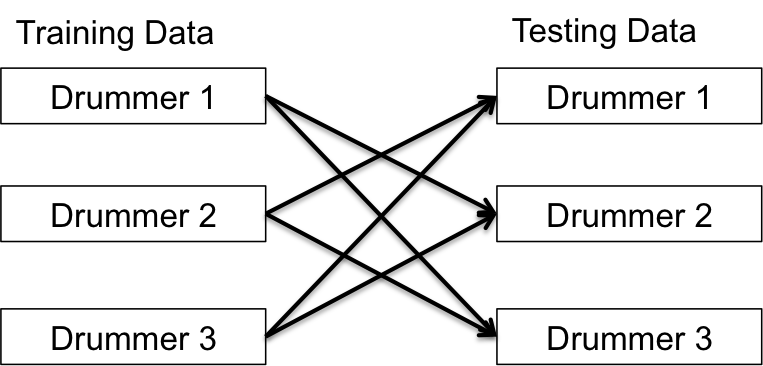
\includegraphics[width=\columnwidth]{cross.png}}}
 \caption{Cross-performer validation process.}
 \label{fig:cross}
\end{figure}

The evaluation metrics follow by the standard calculation of the precision, recall and F-measure as shown in equation \eqref{eq:precision}, equation \eqref{eq:recall} and equation \eqref{eq:Fmeasure}. The $tp$, $fp$, and $fn$ stand for true positive, false positive, and false negative, respectively. A difference within \unit[50]{ms} between the annotated onset and a detected onset is considered as a true positive.  
\begin{equation}
Precision = \frac{tp}{tp + fp}
\label{eq:precision}
\end{equation}

% equation here
\begin{equation}
Recall = \frac{tp}{tp + fn}
\label{eq:recall}
\end{equation}

% equation here
\begin{equation}
F-measure = \frac{2 \times Precision \times Recall}{Precision + Recall}
\label{eq:Fmeasure}
\end{equation}
  



\subsection{Evaluation Results}\label{subsec:evaluation results}

To determine the rank $k$ of the algorithm, $k = {5, 10, 20, 40, 80, 160, 320}$ have been tested. The resulting F-measures of every drum class are shown in \figref{fig:rankTest}. A general trend of performance drop as $k$ increases could be observed, especially for lower frequency sounds such as SD and BD. Based on the trend, a rank number $k = 10$ is chosen in current setup. 

%============= Rank Test Figure
\begin{figure}
 \centerline{\framebox{
 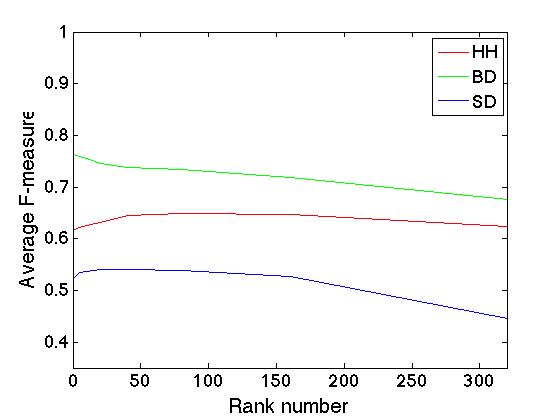
\includegraphics[width=\columnwidth]{rankTest.png}}}
 \caption{Average F-measure versus rank change in harmonic activity matrix.}
 \label{fig:rankTest}
\end{figure}

The results from the first evaluation process is shown in \tabref{tab:basicResults}. There are three experiment setups using the same training data and testing data as mentioned in \ref{subsec:evaluation procedure}. In the first setup, the original signals of the drum samples are used to train the basis matrix, and the original signals from the minus one subset are used as the target signals. The results show that the average F-measure for HH, BD and SD are 0.654, 0.776 and 0.617 respectively. A second setup uses three different filters to pre-process the extracted templates as well as the target signals. A high-pass filter with $f_{hp} = \unit[8000]{Hz}$ is used for HH; a band-pass filter with $f_{bp} = \unit[200--500]{Hz}$ is used for SD; a low-pass filter with $f_{sd} = \unit[150]{Hz}$ is used for BD. The results show that the performance for HH has a significant improvement of 0.702, but the performance for BD and SD drop slightly. Finally, a setup uses only high-pass filter to retain the best overall results has been settled in the current implementation. 

%============= Train on All templates
\begin{table}[h]
\begin{center}
\begin{tabular}{|c|c|c|c|c|}
\hline
\multicolumn{2}{|c|}{}  & Original & HPF+LPF+BPF & HPF only \\ \hline
\multirow{3}{*}{HH} & P & 0.605    & 0.671       & 0.675    \\ \cline{2-5} 
                    & R & 0.713    & 0.737       & 0.736    \\ \cline{2-5} 
                    & F & 0.654    & 0.702       & 0.704    \\ \hline
\multirow{3}{*}{BD} & P & 0.723    & 0.662       & 0.740    \\ \cline{2-5} 
                    & R & 0.837    & 0.855       & 0.839    \\ \cline{2-5} 
                    & F & 0.776    & 0.746       & 0.786    \\ \hline
\multirow{3}{*}{SD} & P & 0.678    & 0.591       & 0.676    \\ \cline{2-5} 
                    & R & 0.566    & 0.583       & 0.569    \\ \cline{2-5} 
                    & F & 0.617    & 0.587       & 0.618    \\ \hline
\end{tabular}
\end{center}
 \caption{Transcription results using all training templates.}
 \label{tab:basicResults}
\end{table}

Another evaluation as described in \figref{fig:cross} has been conducted. Although this process focuses on the exclusiveness between the players, the results of training and testing on the same drummer are still reported in \tabref{tab:trainDr1}, \tabref{tab:trainDr2} and \tabref{tab:trainDr3}. No filters have been applied during the process. In \tabref{tab:trainDr1}, the drum basis matrix is trained on recordings of drummer 1 only. The matrix is then used to decompose polyphonic recordings of different drummers and transcribe drum events. As shown in the table, the testing data from drummer 2 has the best average F-measures of 0.679, 0.842, and 0.691 for HH, BD, and SD.   

%============= Train on Drummer 1 templates
\begin{table}[h]
\begin{center}
\begin{tabular}{|c|c|c|c|c|}
\hline
\multicolumn{2}{|c}{Training} & \multicolumn{3}{|c|}{Drummer 1}   \\ \hline
\multicolumn{2}{|c|}{Testing} & Drummer 1 & Drummer 2 & Drummer 3 \\ \hline
\multirow{3}{*}{HH}    & P    & 0.662     & 0.621     & 0.564     \\ \cline{2-5} 
                       & R    & 0.670     & 0.749     & 0.692     \\ \cline{2-5} 
                       & F    & 0.666     & 0.679     & 0.622     \\ \hline
\multirow{3}{*}{BD}    & P    & 0.620     & 0.781     & 0.850      \\ \cline{2-5} 
                       & R    & 0.393     & 0.914     & 0.900      \\ \cline{2-5} 
                       & F    & 0.481     & 0.842     & 0.874     \\ \hline
\multirow{3}{*}{SD}    & P    & 0.639     & 0.800     & 0.589     \\ \cline{2-5} 
                       & R    & 0.546     & 0.608     & 0.487     \\ \cline{2-5} 
                       & F    & 0.588     & 0.691     & 0.533     \\ \hline
\end{tabular}
 \caption{Transcription results using drummer 1 training templates.}
 \label{tab:trainDr1}
\end{center}
\end{table}

In \tabref{tab:trainDr2}, the drum basis matrix is trained on recordings of drummer 2 only. As shown in the table, the testing data from drummer 2 has the best average F-measures of 0.846, 0.910, and 0.719 for HH, BD, and SD. However, since the basis matrix is trained on the recordings of drummer 2, an improvement of the performance on the same drummer's recording is expected. As for the other drummers, the performance is within the same range.     

%============= Train on Drummer 2 templates
\begin{table}[h]
\begin{center}
\begin{tabular}{|c|c|c|c|c|}
\hline
\multicolumn{2}{|c}{Training} & \multicolumn{3}{|c|}{Drummer 2}   \\ \hline
\multicolumn{2}{|c|}{Testing} & Drummer 1 & Drummer 2 & Drummer 3 \\ \hline
\multirow{3}{*}{HH}    & P    & 0.661     & 0.600     & 0.541     \\ \cline{2-5} 
                       & R    & 0.667     & 0.787     & 0.699     \\ \cline{2-5} 
                       & F    & 0.664     & 0.681     & 0.610     \\ \hline
\multirow{3}{*}{BD}    & P    & 0.466     & 0.846     & 0.699     \\ \cline{2-5} 
                       & R    & 0.603     & 0.986     & 0.854     \\ \cline{2-5} 
                       & F    & 0.525     & 0.910     & 0.769     \\ \hline
\multirow{3}{*}{SD}    & P    & 0.625     & 0.849     & 0.529     \\ \cline{2-5} 
                       & R    & 0.550     & 0.624     & 0.486     \\ \cline{2-5} 
                       & F    & 0.585     & 0.719     & 0.506     \\ \hline
\end{tabular}
 \caption{Transcription results using drummer 2 training templates.}
 \label{tab:trainDr2}
\end{center}
\end{table}

Finally, in \tabref{tab:trainDr3}, the drum basis matrix is trained on recordings of drummer 3 only. As shown in the table, the testing data from drummer 2 has the best average F-measures of 0.862, 0.910, and 0.607 for HH, BD, and SD. In general, the testing data from drummer 2 has the best overall performance with different training data from all the drummers. Besides, all the results have a similar trend no matter which training data is used. This result might imply that this algorithm is less template dependent, allowing a general use case where a drum template could be constructed from different sound sources and be applied to different polyphonic recordings. However, the performance of this setup still needs to be confirmed with a cross-dataset validation.      

%============= Train on Drummer 3 templates
\begin{table}[h]
\begin{center}
\begin{tabular}{|c|c|c|c|c|}
\hline
\multicolumn{2}{|c}{Training} & \multicolumn{3}{|c|}{Drummer 3}   \\ \hline
\multicolumn{2}{|c|}{Testing} & Drummer 1 & Drummer 2 & Drummer 3 \\ \hline
\multirow{3}{*}{HH}    & P    & 0.614     & 0.599     & 0.523     \\ \cline{2-5} 
                       & R    & 0.660     & 0.717     & 0.675     \\ \cline{2-5} 
                       & F    & 0.636     & 0.652     & 0.589     \\ \hline
\multirow{3}{*}{BD}    & P    & 0.506     & 0.862     & 0.800     \\ \cline{2-5} 
                       & R    & 0.636     & 0.965     & 0.932     \\ \cline{2-5} 
                       & F    & 0.564     & 0.910     & 0.861     \\ \hline
\multirow{3}{*}{SD}    & P    & 0.477     & 0.615     & 0.564     \\ \cline{2-5} 
                       & R    & 0.580     & 0.598     & 0.534     \\ \cline{2-5} 
                       & F    & 0.523     & 0.607     & 0.548     \\ \hline
\end{tabular}
 \caption{Transcription results using drummer 3 training templates.}
 \label{tab:trainDr3}
\end{center}
\end{table}

\section{Conclusion}\label{sec:Conclusion}

In this paper, a drum transcription system in polyphonic music using semi-supervised NMF has been presented. This method uses a pre-trained drum basis matrix to decompose the target signal, extract the drum activity matrix, and adapt the harmonic parts. This NMF based method for drum transcription task has some advantages over instance-based methods: firstly, the simultaneous sounds could be detected separately. Normally, when more classes of drums are being considered in a instance-based transcription task, more combination of classes need to be considered, and the situation could be more complicated. With a NMF approach, there is no need to train more classes to handle such situations. Secondly, the parameter $k$ allows the algorithm to adapt to different content of polyphonic music and could potentially improve the performance of the basic NMF approach in the context of polyphonic music. This evaluation results show that this method is able to achieve 61~77\% accuracy in polyphonic music. Furthermore, the results from the cross-performer validation indicate that this method still apply to the situations when minimum prior knowledge about the drum sounds in the target signal is given.

To achieve a complete drum transcription system in polyphonic music, however, more factors such as playing techniques and different drum setups still need to be addressed in the future. 

Dummycite: \cite{tzanetakis_musical_2002}

%\section{Reference}
%
%
%% I haven't done this part yet...
%
%
%
%%============= This part is for reference only, will be removed once my parts are finished =============
%\section{Equations}
%
%Equations should be placed on separated lines and numbered.
%The number should be on the right side, in parentheses.
%
%\begin{equation}
%E=mc^{2}
%\end{equation}

%\section{Citations}
%
%All bibliographical references should be listed at the end,
%inside a section named ``REFERENCES,'' numbered and in alphabetical order.
%Also, all references listed should be cited in the text.
%When referring to a document, type the numbering square brackets
%\cite{Author:00} or \cite{Author:00,Someone:10,Someone:04}.
%
%\begin{thebibliography}{citations}
%
%\bibitem {Author:00}
%E. Author:
%``The Title of the Conference Paper,''
%{\it Proceedings of the International Symposium
%on Music Information Retrieval}, pp.~000--111, 2000.
%
%\bibitem{Someone:10}
%A. Someone, B. Someone, and C. Someone:
%``The Title of the Journal Paper,''
%{\it Journal of New Music Research},
%Vol.~A, No.~B, pp.~111--222, 2010.
%
%\bibitem{Someone:04} X. Someone and Y. Someone: {\it Title of the Book},
    %Editorial Acme, Porto, 2012.
%
%\end{thebibliography}

\bibliography{ismir2014template}

\end{document}
